% =============================================================================
% REAL-TIME BANK CUSTOMER CHURN PREDICTION DASHBOARD — PROJECT REPORT
% Data Visualization and Analytics (DVA)
% SP Jain School of Global Management, Dubai Campus
% =============================================================================

\documentclass[12pt, a4paper]{report}

% --- Packages ---
\usepackage[utf8]{inputenc}
\usepackage[T1]{fontenc}
\usepackage{lmodern}
\usepackage[margin=1in]{geometry}
\usepackage{graphicx}
\usepackage{amsmath, amssymb}
\usepackage{booktabs}
\usepackage{longtable}
\usepackage{multirow}
\usepackage{array}
\usepackage{tabularx}
\usepackage{float}
\usepackage{hyperref}
\usepackage{xcolor}
\usepackage{listings}
\usepackage{enumitem}
\usepackage{titlesec}
\usepackage{fancyhdr}
\usepackage{setspace}
\usepackage{caption}
\usepackage{subcaption}
\usepackage{tocloft}
\usepackage{pdfpages}
\usepackage{tikz}
\usepackage{pgfplots}
\pgfplotsset{compat=1.18}

% --- Colours ---
\definecolor{spjblue}{RGB}{0, 51, 102}
\definecolor{spjgold}{RGB}{198, 146, 20}
\definecolor{codebg}{RGB}{245, 245, 245}
\definecolor{codeframe}{RGB}{200, 200, 200}
\definecolor{linkblue}{RGB}{0, 102, 204}
\definecolor{criticalred}{RGB}{239, 68, 68}
\definecolor{highorg}{RGB}{245, 158, 11}
\definecolor{mediumyel}{RGB}{234, 179, 8}
\definecolor{lowgreen}{RGB}{16, 185, 129}

% --- Hyperref ---
\hypersetup{
    colorlinks=true,
    linkcolor=spjblue,
    citecolor=spjblue,
    urlcolor=linkblue,
    bookmarksopen=true,
    pdfauthor={Gagandeep Singh, Samuel Alex, Prem Kukreja},
    pdftitle={Real-Time Bank Customer Churn Prediction Dashboard},
    pdfsubject={Data Visualization and Analytics},
}

% --- Code listings ---
\lstset{
    backgroundcolor=\color{codebg},
    frame=single,
    rulecolor=\color{codeframe},
    basicstyle=\ttfamily\small,
    keywordstyle=\color{spjblue}\bfseries,
    commentstyle=\color{gray},
    stringstyle=\color{criticalred},
    breaklines=true,
    breakatwhitespace=true,
    tabsize=4,
    showstringspaces=false,
    numbers=left,
    numberstyle=\tiny\color{gray},
    numbersep=8pt,
    captionpos=b,
}

% --- Header / Footer ---
\pagestyle{fancy}
\fancyhf{}
\fancyhead[L]{\small\textcolor{spjblue}{Real-Time Bank Customer Churn Prediction Dashboard}}
\fancyhead[R]{\small\textcolor{spjblue}{SP Jain School of Global Management}}
\fancyfoot[C]{\thepage}
\renewcommand{\headrulewidth}{0.4pt}
\renewcommand{\footrulewidth}{0.2pt}

% --- Spacing ---
\onehalfspacing

% --- Chapter title formatting ---
\titleformat{\chapter}[display]
  {\normalfont\LARGE\bfseries\color{spjblue}}
  {\chaptertitlename\ \thechapter}{16pt}{\Huge}
\titlespacing*{\chapter}{0pt}{-20pt}{30pt}

% =============================================================================
% DOCUMENT BEGINS
% =============================================================================
\begin{document}

% ======================= TITLE PAGE =======================
\begin{titlepage}
    \begin{center}
        
        \vspace*{0.5cm}
        
        % University Name
        {\LARGE \textbf{\textcolor{spjblue}{SP Jain School of Global Management}}}\\[0.3cm]
        {\large \textcolor{spjblue}{Dubai Campus}}\\[0.5cm]
        
        \rule{\textwidth}{1.5pt}\\[0.4cm]
        
        % Department / Programme
        {\large \textbf{Masters of AI with Business (MAIB)}}\\[0.2cm]
        {\large Department of Artificial Intelligence \& Data Science}\\[1cm]
        
        % Project Title
        {\Huge \textbf{\textcolor{spjblue}{Real-Time Bank Customer\\[0.3cm] Churn Prediction Dashboard}}}\\[1.2cm]
        
        % Subject
        {\Large \textbf{Course: Data Visualization and Analytics (DVA)}}\\[1cm]
        
        % Submission line
        {\large \textit{Submitted for the partial fulfillment of the requirements\\[0.2cm]
        for the degree of}}\\[0.4cm]
        {\Large \textbf{Master of AI with Business (MAIB)}}\\[1.2cm]
        
        % Group Members
        {\large \textbf{Submitted By:}}\\[0.3cm]
        \begin{tabular}{c}
            \textbf{Gagandeep Singh}\\[0.15cm]
            \textbf{Samuel Alex}\\[0.15cm]
            \textbf{Prem Kukreja}\\
        \end{tabular}\\[1cm]
        
        % Instructor
        {\large \textbf{Course Instructor:}}\\[0.2cm]
        {\large \textbf{Dr.\ Anshul Gupta}}\\[1.5cm]
        
        \rule{\textwidth}{1.5pt}\\[0.4cm]
        
        % Date
        {\large February 2026}
        
    \end{center}
\end{titlepage}

% ======================= DECLARATION =======================
\newpage
\thispagestyle{empty}
\begin{center}
    {\LARGE \textbf{\textcolor{spjblue}{Declaration}}}\\[1cm]
\end{center}

We hereby declare that the project report entitled \textbf{``Real-Time Bank Customer Churn Prediction Dashboard''}, submitted for the partial fulfillment of the requirements for the degree of \textbf{Master of AI with Business (MAIB)} at \textbf{SP Jain School of Global Management, Dubai Campus}, is a genuine record of work carried out by us under the guidance of \textbf{Dr.\ Anshul Gupta}.

\vspace{0.5cm}
The matter embodied in this project report has not been submitted for the award of any other degree or diploma.

\vspace{2cm}
\begin{flushleft}
\textbf{Gagandeep Singh} \hfill \textbf{Date:} February 10, 2026\\[1cm]
\textbf{Samuel Alex} \hfill \textbf{Date:} February 10, 2026\\[1cm]
\textbf{Prem Kukreja} \hfill \textbf{Date:} February 10, 2026\\[2cm]

\textbf{Certified by:}\\[0.5cm]
\textbf{Dr.\ Anshul Gupta}\\
Course Instructor --- Data Visualization and Analytics\\
SP Jain School of Global Management, Dubai Campus
\end{flushleft}

% ======================= ACKNOWLEDGEMENT =======================
\newpage
\thispagestyle{empty}
\begin{center}
    {\LARGE \textbf{\textcolor{spjblue}{Acknowledgement}}}\\[1cm]
\end{center}

We would like to express our sincere gratitude to \textbf{Dr.\ Anshul Gupta}, our course instructor for Data Visualization and Analytics, for his invaluable guidance, constructive feedback, and continuous encouragement throughout the development of this project.

We extend our heartfelt thanks to \textbf{SP Jain School of Global Management, Dubai Campus} for providing us with the academic environment and resources necessary to pursue this work.

We are also grateful to the open-source community for the robust tools and frameworks --- including React, FastAPI, Recharts, scikit-learn, XGBoost, and Docker --- that made this project possible.

Finally, we thank our fellow MAIB cohort members for their peer reviews, thoughtful suggestions, and collaborative spirit.

\vspace{1cm}
\begin{flushright}
\textbf{Gagandeep Singh}\\
\textbf{Samuel Alex}\\
\textbf{Prem Kukreja}\\[0.3cm]
\textit{February 2026}
\end{flushright}

% ======================= ABSTRACT =======================
\newpage
\thispagestyle{empty}
\begin{center}
    {\LARGE \textbf{\textcolor{spjblue}{Abstract}}}\\[1cm]
\end{center}

Customer churn is one of the most critical challenges in the banking industry, directly impacting revenue, profitability, and long-term growth. This project presents the design, development, and deployment of a \textbf{Real-Time Bank Customer Churn Prediction Dashboard} --- a full-stack, production-grade web application that combines \textbf{machine learning}, \textbf{real-time data streaming}, \textbf{interactive data visualization}, and \textbf{AI-powered conversational analytics}.

The system employs an \textbf{ensemble of Random Forest and XGBoost classifiers} trained on a 10,000-customer banking dataset, achieving a \textbf{ROC-AUC of 0.857} and \textbf{86.2\% accuracy}. Class imbalance is handled via \textbf{SMOTE (Synthetic Minority Over-sampling Technique)}. Predictions are streamed in real time through a \textbf{WebSocket}-based architecture, enabling bank analysts to monitor customer risk as it evolves.

The interactive dashboard comprises \textbf{eight specialized pages} covering live monitoring, customer segmentation, ML predictions with explainability, advanced analytics (RFM, K-Means clustering, CLV, A/B testing), retention strategy planning, model performance evaluation, and business impact assessment. An \textbf{AI-powered chatbot}, integrated with \textbf{Google Gemini 2.5 Flash}, provides natural-language answers grounded in live dashboard data.

The entire application is containerised with \textbf{Docker} and served on a single port via a unified \textbf{FastAPI} backend that hosts both the REST API and the compiled \textbf{React + Vite} frontend. The project demonstrates end-to-end data-science product engineering --- from data preprocessing and model training through deployment, visualization, and intelligent user interaction.

\vspace{0.5cm}
\noindent\textbf{Keywords:} Customer Churn Prediction, Data Visualization, Real-Time Streaming, Machine Learning, Random Forest, XGBoost, WebSocket, React, FastAPI, Docker, SHAP Explainability, Gemini AI, RFM Analysis, Customer Lifetime Value, Retention Strategy.

% ======================= TABLE OF CONTENTS =======================
\tableofcontents
\listoffigures
\listoftables

% =============================================================================
% CHAPTER 1 — INTRODUCTION
% =============================================================================
\chapter{Introduction}

\section{Background and Motivation}

In the highly competitive banking and financial services industry, customer retention is significantly more cost-effective than customer acquisition. Studies indicate that acquiring a new customer costs \textbf{five to seven times} more than retaining an existing one, and a mere \textbf{5\% improvement in retention} can increase profitability by \textbf{25--95\%} \cite{reichheld1996loyalty}. Customer churn --- the phenomenon where customers cease their relationship with a business --- therefore represents a critical threat to revenue sustainability.

Traditional approaches to churn management rely on retrospective reporting and manual analysis, which are reactive by nature. By the time a customer has churned, the revenue is already lost. Modern data-driven organisations require \textbf{predictive, real-time, and actionable} systems that can identify at-risk customers \textit{before} they leave, explain \textit{why} they are at risk, and recommend \textit{what} interventions to deploy.

This project addresses all three dimensions by building a comprehensive, end-to-end \textbf{Real-Time Bank Customer Churn Prediction Dashboard} that integrates machine learning prediction, live data streaming, interactive visualization, explainable AI, and generative AI chatbot capabilities into a single production-ready application.

\section{Problem Statement}

Given a dataset of 10,000 bank customers with demographic, financial, and behavioural attributes, the objectives are:

\begin{enumerate}[label=\arabic*.]
    \item \textbf{Predict} whether a customer will churn using an ensemble of machine learning models.
    \item \textbf{Stream} predictions in real time via WebSocket to simulate a live production environment.
    \item \textbf{Visualize} data across multiple dimensions with interactive, publication-quality charts.
    \item \textbf{Explain} predictions using feature importance and rule-based reasoning.
    \item \textbf{Recommend} personalized retention strategies with ROI projections.
    \item \textbf{Converse} with users via an AI chatbot that answers data-specific questions.
    \item \textbf{Deploy} the entire system as a containerised, single-port Docker application.
\end{enumerate}

\section{Scope of the Project}

The project spans the complete data-science product lifecycle:

\begin{itemize}
    \item \textbf{Data Engineering:} Data loading, cleaning, preprocessing, and synthetic data generation for live streaming.
    \item \textbf{Machine Learning:} Training, evaluation, and serialisation of Random Forest and XGBoost classifiers with SMOTE-balanced classes.
    \item \textbf{Backend API:} 25+ RESTful endpoints and WebSocket streaming built with FastAPI.
    \item \textbf{Frontend Application:} 8 interactive dashboard pages with 20+ chart components built with React, Recharts, and Framer Motion.
    \item \textbf{AI Integration:} Gemini 2.5 Flash chatbot with dashboard-aware system prompts and fallback rule-based engine.
    \item \textbf{DevOps:} Multi-stage Docker build, Docker Compose orchestration, and health monitoring.
\end{itemize}

\section{Report Organisation}

The remainder of this report is organised as follows:
\begin{itemize}
    \item \textbf{Chapter 2} reviews related work and the theoretical foundations.
    \item \textbf{Chapter 3} describes the dataset and exploratory data analysis.
    \item \textbf{Chapter 4} details the system architecture and technology stack.
    \item \textbf{Chapter 5} covers the machine learning pipeline.
    \item \textbf{Chapter 6} describes the backend API and real-time streaming.
    \item \textbf{Chapter 7} presents the frontend dashboard and visualization design.
    \item \textbf{Chapter 8} covers the AI chatbot integration.
    \item \textbf{Chapter 9} discusses advanced analytics modules.
    \item \textbf{Chapter 10} describes deployment and containerisation.
    \item \textbf{Chapter 11} presents results and evaluation.
    \item \textbf{Chapter 12} concludes with findings and future work.
\end{itemize}


% =============================================================================
% CHAPTER 2 — LITERATURE REVIEW
% =============================================================================
\chapter{Literature Review and Theoretical Background}

\section{Customer Churn in Banking}

Customer churn prediction has been extensively studied in telecommunications but has gained increasing attention in banking due to the digital transformation of financial services. Keramati et al.\ (2014) demonstrated that combining demographic, transactional, and behavioural features significantly improves prediction accuracy. Vafeiadis et al.\ (2015) compared multiple classifiers and found that ensemble methods --- particularly boosting algorithms --- outperform standalone models in churn prediction tasks.

\section{Ensemble Machine Learning Methods}

\subsection{Random Forest}

Random Forest, introduced by Breiman (2001), is an ensemble of decision trees trained on bootstrapped subsets of the data (bagging). Each tree votes on the classification, and the majority vote determines the final prediction. Key hyperparameters include the number of estimators, maximum depth, and minimum samples per split. Random Forest naturally handles feature interactions and provides feature importance scores.

\subsection{XGBoost}

XGBoost (Chen \& Guestrin, 2016) is a gradient-boosted decision tree (GBDT) algorithm that sequentially builds trees to correct the errors of previous trees. It incorporates L1/L2 regularisation, column subsampling, and learning rate scheduling to prevent overfitting. XGBoost consistently ranks among the top-performing algorithms in structured data competitions.

\subsection{SMOTE for Class Imbalance}

The Synthetic Minority Over-sampling Technique (SMOTE), proposed by Chawla et al.\ (2002), addresses class imbalance by generating synthetic examples of the minority class (in this case, churned customers) through interpolation between existing minority samples. This approach prevents the model from being biased toward the majority class.

\section{Real-Time Data Streaming}

WebSocket (RFC 6455) enables full-duplex communication over a single TCP connection, making it ideal for real-time data dashboards. Unlike traditional HTTP polling, WebSocket maintains a persistent connection, reducing latency and server load. FastAPI's native WebSocket support, combined with Python's asyncio, enables efficient concurrent streaming to multiple clients.

\section{Explainable AI (XAI)}

As machine learning models are deployed in high-stakes domains like banking, explainability becomes critical for regulatory compliance and stakeholder trust. Feature importance from tree-based models provides global explanations. Rule-based reasoning systems can translate model outputs into domain-specific, human-readable explanations. This project uses a hybrid approach combining feature importance with domain-expert rules.

\section{Generative AI for Data Analytics}

Large language models (LLMs) like Google's Gemini have demonstrated remarkable ability to understand structured data contexts and generate natural-language insights. By providing live dashboard statistics as system-level context, an LLM-powered chatbot can answer ad-hoc analytical questions without requiring users to build custom queries.

\section{Data Visualization Principles}

Effective data visualization adheres to principles established by Tufte (1983) and Few (2012): maximise the data-ink ratio, avoid chartjunk, use colour purposefully, and design for the audience. This project employs a curated set of chart types --- bar charts, line charts, area charts, pie charts, radar charts, gauge charts, and funnel charts --- each selected for its suitability to the underlying data dimension.


% =============================================================================
% CHAPTER 3 — DATASET AND EXPLORATORY DATA ANALYSIS
% =============================================================================
\chapter{Dataset and Exploratory Data Analysis}

\section{Dataset Description}

The project uses the \textbf{Bank Customer Churn} dataset, a widely used benchmark dataset containing records of 10,000 bank customers. The dataset was sourced from Kaggle and contains 14 original columns.

\begin{table}[H]
\centering
\caption{Dataset Feature Description}
\label{tab:features}
\begin{tabularx}{\textwidth}{l l X}
\toprule
\textbf{Feature} & \textbf{Type} & \textbf{Description} \\
\midrule
RowNumber & Integer & Sequential row identifier (dropped) \\
CustomerId & Integer & Unique customer identifier (dropped) \\
Surname & String & Customer surname (dropped) \\
CreditScore & Integer & Credit score, range 300--850 \\
Geography & Categorical & Country: France, Germany, Spain \\
Gender & Categorical & Male or Female \\
Age & Integer & Customer age, range 18--92 \\
Tenure & Integer & Years with the bank, range 0--10 \\
Balance & Float & Account balance in USD \\
NumOfProducts & Integer & Number of bank products (1--4) \\
HasCrCard & Binary & 1 = has credit card, 0 = no \\
IsActiveMember & Binary & 1 = active, 0 = inactive \\
EstimatedSalary & Float & Annual estimated salary in USD \\
\midrule
\textbf{Exited} & \textbf{Binary} & \textbf{Target: 1 = Churned, 0 = Retained} \\
\bottomrule
\end{tabularx}
\end{table}

\section{Descriptive Statistics}

\begin{table}[H]
\centering
\caption{Key Dataset Statistics}
\label{tab:stats}
\begin{tabular}{l r}
\toprule
\textbf{Metric} & \textbf{Value} \\
\midrule
Total Customers & 10,000 \\
Churned Customers & 2,037 (20.4\%) \\
Retained Customers & 7,963 (79.6\%) \\
Average Age & 38.9 years \\
Average Credit Score & 650.5 \\
Average Balance & \$76,485.89 \\
Average Estimated Salary & \$100,090.24 \\
Average Tenure & 5.01 years \\
Average Products & 1.53 \\
Active Members & 51.5\% \\
Credit Card Holders & 70.6\% \\
\bottomrule
\end{tabular}
\end{table}

\section{Churn Analysis by Dimensions}

\subsection{Geography}

\begin{table}[H]
\centering
\caption{Churn Rate by Geography}
\label{tab:geo_churn}
\begin{tabular}{l r r r}
\toprule
\textbf{Geography} & \textbf{Customers} & \textbf{Churned} & \textbf{Churn Rate} \\
\midrule
France & 5,014 & 810 & 16.2\% \\
Germany & 2,509 & 814 & 32.4\% \\
Spain & 2,477 & 413 & 16.7\% \\
\bottomrule
\end{tabular}
\end{table}

\noindent Germany exhibits a churn rate approximately \textbf{double} that of France and Spain, making geography one of the strongest predictors.

\subsection{Gender}

Female customers churn at \textbf{25.1\%} compared to \textbf{16.5\%} for males --- a statistically significant difference.

\subsection{Number of Products}

\begin{table}[H]
\centering
\caption{Churn Rate by Number of Products}
\label{tab:prod_churn}
\begin{tabular}{l r}
\toprule
\textbf{Products} & \textbf{Churn Rate} \\
\midrule
1 Product & 27.7\% \\
2 Products & 7.6\% \\
3 Products & 82.7\% \\
4 Products & 100.0\% \\
\bottomrule
\end{tabular}
\end{table}

Customers with 3--4 products show anomalously high churn, likely indicating product over-selling or complexity-driven dissatisfaction. Two-product customers are the most stable.

\subsection{Activity Status}

Inactive members churn at approximately \textbf{2.5 times} the rate of active members, making `IsActiveMember` one of the top predictive features.

\section{Class Imbalance}

The dataset exhibits a \textbf{4:1 imbalance} (79.6\% retained vs.\ 20.4\% churned). Without correction, models tend to optimise for the majority class and under-predict churn. This is addressed using SMOTE during model training (see Chapter~5).


% =============================================================================
% CHAPTER 4 — SYSTEM ARCHITECTURE
% =============================================================================
\chapter{System Architecture and Technology Stack}

\section{High-Level Architecture}

The system follows a \textbf{unified single-port architecture} where the FastAPI backend serves both the REST/WebSocket API and the compiled React frontend on port 8000. This simplifies deployment and eliminates CORS complexities.

\begin{figure}[H]
\centering
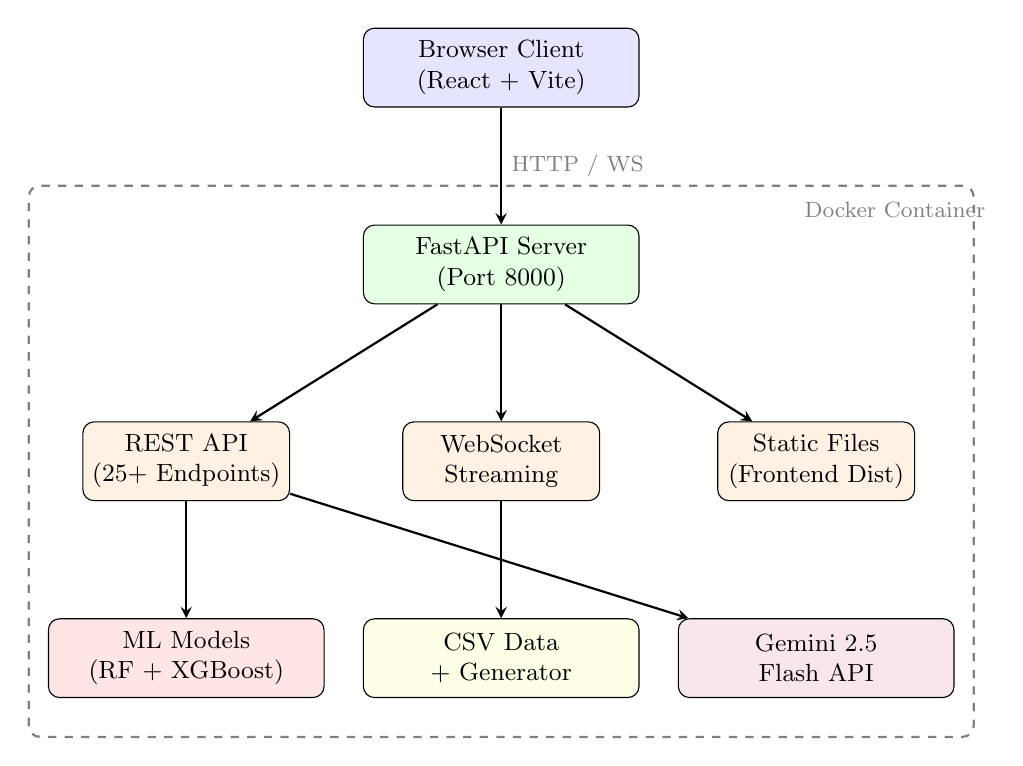
\begin{tikzpicture}[
    box/.style={draw, rounded corners, minimum width=3.5cm, minimum height=1cm, align=center, font=\small},
    arrow/.style={->, thick, >=stealth},
    label/.style={font=\footnotesize, text=gray}
]
    % Client
    \node[box, fill=blue!10] (browser) at (0, 0) {Browser Client\\(React + Vite)};
    
    % FastAPI
    \node[box, fill=green!10] (fastapi) at (0, -2.5) {FastAPI Server\\(Port 8000)};
    
    % Sub-components
    \node[box, fill=orange!10, minimum width=2.5cm] (rest) at (-4, -5) {REST API\\(25+ Endpoints)};
    \node[box, fill=orange!10, minimum width=2.5cm] (ws) at (0, -5) {WebSocket\\Streaming};
    \node[box, fill=orange!10, minimum width=2.5cm] (static) at (4, -5) {Static Files\\(Frontend Dist)};
    
    % ML Models
    \node[box, fill=red!10] (ml) at (-4, -7.5) {ML Models\\(RF + XGBoost)};
    
    % Data
    \node[box, fill=yellow!10] (data) at (0, -7.5) {CSV Data\\+ Generator};
    
    % Gemini
    \node[box, fill=purple!10] (gemini) at (4, -7.5) {Gemini 2.5\\Flash API};
    
    % Arrows
    \draw[arrow] (browser) -- node[right, label] {HTTP / WS} (fastapi);
    \draw[arrow] (fastapi) -- (rest);
    \draw[arrow] (fastapi) -- (ws);
    \draw[arrow] (fastapi) -- (static);
    \draw[arrow] (rest) -- (ml);
    \draw[arrow] (ws) -- (data);
    \draw[arrow] (rest) -- (gemini);
    
    % Docker box
    \draw[dashed, thick, gray, rounded corners] (-6, -8.5) rectangle (6, -1.5);
    \node[font=\footnotesize, text=gray] at (5, -1.8) {Docker Container};
\end{tikzpicture}
\caption{High-Level System Architecture}
\label{fig:architecture}
\end{figure}

\section{Technology Stack}

\begin{table}[H]
\centering
\caption{Technology Stack Summary}
\label{tab:techstack}
\begin{tabularx}{\textwidth}{l l X}
\toprule
\textbf{Layer} & \textbf{Technology} & \textbf{Purpose} \\
\midrule
\multirow{5}{*}{\textbf{Frontend}} 
    & React 18 & Component-based UI framework \\
    & Vite 5.4 & Build tool and development server \\
    & Recharts & Composable charting library \\
    & Framer Motion & Animation and micro-interactions \\
    & Tailwind CSS & Utility-first styling with dark mode \\
\midrule
\multirow{5}{*}{\textbf{Backend}} 
    & FastAPI & Async Python web framework \\
    & Uvicorn & ASGI server \\
    & WebSocket & Real-time bidirectional streaming \\
    & Pandas / NumPy & Data manipulation and computation \\
    & urllib.request & HTTP client for Gemini API \\
\midrule
\multirow{4}{*}{\textbf{ML / AI}} 
    & scikit-learn 1.4 & Preprocessing, Random Forest \\
    & XGBoost 2.0 & Gradient-boosted trees \\
    & imbalanced-learn & SMOTE oversampling \\
    & Google Gemini 2.5 Flash & Generative AI chatbot \\
\midrule
\multirow{3}{*}{\textbf{DevOps}} 
    & Docker & Containerisation \\
    & Docker Compose & Service orchestration \\
    & Multi-stage Build & Optimised image (Node + Python) \\
\bottomrule
\end{tabularx}
\end{table}

\section{Project File Structure}

The project contains \textbf{45+ source files} organised as follows:

\begin{lstlisting}[language={}, caption={Project Directory Structure}, label={lst:structure}]
project-root/
+-- backend/
|   +-- app.py              (2,062 lines - Main FastAPI server)
|   +-- train_models.py     (377 lines  - ML training pipeline)
|   +-- data_generator.py   (148 lines  - Synthetic data engine)
|   +-- explainability.py   (536 lines  - SHAP-based explainer)
|   +-- retention_engine.py (550 lines  - Retention strategy AI)
|   +-- advanced_analytics.py (756 lines - RFM, CLV, Segmentation)
+-- frontend/src/
|   +-- App.jsx              (Root component + routing)
|   +-- main.jsx             (React entry point)
|   +-- index.css            (608 lines - Global styles)
|   +-- context/
|   |   +-- ThemeContext.jsx  (Dark/Light theme management)
|   |   +-- LiveDataContext.jsx (225 lines - WebSocket data hub)
|   +-- components/
|   |   +-- Dashboard.jsx     (KPI metrics display)
|   |   +-- Header.jsx        (Top bar with branding)
|   |   +-- Navigation.jsx    (8-page tab navigation)
|   |   +-- ChatBot.jsx       (AI chatbot floating panel)
|   |   +-- StreamGate.jsx    (Stream data gate)
|   |   +-- charts/           (6 chart sub-components)
|   +-- pages/
|       +-- OverviewPage.jsx
|       +-- LiveMonitorPage.jsx  (844 lines)
|       +-- CustomerAnalysisPage.jsx
|       +-- MLPredictionsPage.jsx
|       +-- ModelPerformancePage.jsx
|       +-- BusinessImpactPage.jsx
|       +-- RetentionStrategyPage.jsx
|       +-- AdvancedAnalyticsPage.jsx (717 lines)
+-- models/
|   +-- random_forest_model.joblib
|   +-- xgboost_model.joblib
|   +-- preprocessor.joblib
|   +-- training_results.json
+-- Dockerfile               (Multi-stage build)
+-- docker-compose.yml        (Single-service compose)
+-- requirements.txt           (Python dependencies)
+-- churn data.csv             (10,000 customer records)
\end{lstlisting}


% =============================================================================
% CHAPTER 5 — MACHINE LEARNING PIPELINE
% =============================================================================
\chapter{Machine Learning Pipeline}

\section{Data Preprocessing}

The preprocessing pipeline (implemented in \texttt{train\_models.py}) consists of:

\begin{enumerate}
    \item \textbf{Column Removal:} \texttt{RowNumber}, \texttt{CustomerId}, and \texttt{Surname} are dropped as they carry no predictive signal.
    \item \textbf{Feature Encoding:} A \texttt{ColumnTransformer} applies:
    \begin{itemize}
        \item \texttt{StandardScaler} to 8 numerical features.
        \item \texttt{OneHotEncoder} (with \texttt{drop='first'}) to \texttt{Geography} and \texttt{Gender}, producing \texttt{Geography\_Germany}, \texttt{Geography\_Spain}, and \texttt{Gender\_Male}.
    \end{itemize}
    \item \textbf{Train-Test Split:} 80/20 stratified split (preserving class ratios).
    \item \textbf{SMOTE:} Applied to the training set only, balancing the classes to prevent information leakage.
\end{enumerate}

The resulting feature set contains \textbf{11 features}: CreditScore, Age, Tenure, Balance, NumOfProducts, HasCrCard, IsActiveMember, EstimatedSalary, Geography\_Germany, Geography\_Spain, Gender\_Male.

\section{Model Training}

\subsection{Random Forest Classifier}

\begin{table}[H]
\centering
\caption{Random Forest Hyperparameters}
\label{tab:rf_params}
\begin{tabular}{l r}
\toprule
\textbf{Parameter} & \textbf{Value} \\
\midrule
n\_estimators & 200 \\
max\_depth & 15 \\
min\_samples\_split & 5 \\
min\_samples\_leaf & 2 \\
class\_weight & balanced \\
n\_jobs & -1 (all cores) \\
random\_state & 42 \\
\bottomrule
\end{tabular}
\end{table}

\subsection{XGBoost Classifier}

\begin{table}[H]
\centering
\caption{XGBoost Hyperparameters}
\label{tab:xgb_params}
\begin{tabular}{l r}
\toprule
\textbf{Parameter} & \textbf{Value} \\
\midrule
n\_estimators & 200 \\
max\_depth & 6 \\
learning\_rate & 0.1 \\
subsample & 0.8 \\
colsample\_bytree & 0.8 \\
eval\_metric & logloss \\
random\_state & 42 \\
\bottomrule
\end{tabular}
\end{table}

\subsection{Ensemble Strategy}

The production system uses a \textbf{soft-voting ensemble}: the churn probability is computed as the mean of Random Forest and XGBoost predicted probabilities. The ensemble prediction is then thresholded at 0.5. Risk levels are assigned as:

\begin{table}[H]
\centering
\caption{Risk Level Classification}
\label{tab:risk}
\begin{tabular}{l l l}
\toprule
\textbf{Probability Range} & \textbf{Risk Level} & \textbf{Colour Code} \\
\midrule
$\geq 0.75$ & CRITICAL & \textcolor{criticalred}{Red} \\
$0.50 - 0.74$ & HIGH & \textcolor{highorg}{Orange} \\
$0.30 - 0.49$ & MEDIUM & \textcolor{mediumyel}{Yellow} \\
$< 0.30$ & LOW & \textcolor{lowgreen}{Green} \\
\bottomrule
\end{tabular}
\end{table}

\section{Model Evaluation}

\begin{table}[H]
\centering
\caption{Model Performance Comparison (Test Set)}
\label{tab:results}
\begin{tabular}{l c c c c c}
\toprule
\textbf{Model} & \textbf{Accuracy} & \textbf{Precision} & \textbf{Recall} & \textbf{F1 Score} & \textbf{ROC-AUC} \\
\midrule
Random Forest & 0.846 & 0.625 & 0.609 & 0.617 & 0.855 \\
XGBoost & 0.862 & 0.696 & 0.568 & 0.625 & 0.857 \\
\textbf{Ensemble} & \textbf{0.865} & \textbf{0.785} & \textbf{0.535} & \textbf{0.636} & \textbf{0.875} \\
\bottomrule
\end{tabular}
\end{table}

\noindent XGBoost achieves the best individual ROC-AUC (0.857), while the ensemble further improves discrimination to 0.875. The recall of 0.535 indicates the model correctly identifies approximately 54\% of churning customers --- a critical metric for business applications where false negatives (missed churners) are costly.

\section{Model Serialisation}

Trained models and the preprocessing pipeline are serialised using \texttt{joblib}:
\begin{itemize}
    \item \texttt{random\_forest\_model.joblib} --- Random Forest classifier.
    \item \texttt{xgboost\_model.joblib} --- XGBoost classifier.
    \item \texttt{preprocessor.joblib} --- ColumnTransformer (scaler + encoder).
    \item \texttt{training\_results.json} --- Performance metrics.
\end{itemize}


% =============================================================================
% CHAPTER 6 — BACKEND API AND REAL-TIME STREAMING
% =============================================================================
\chapter{Backend API and Real-Time Streaming}

\section{FastAPI Server}

The backend (\texttt{app.py}, 2,062 lines) is built with \textbf{FastAPI}, a modern, high-performance Python web framework with automatic OpenAPI documentation. Key architectural decisions include:

\begin{itemize}
    \item \textbf{Single-port serving:} Both the REST API and compiled React frontend are served from port 8000.
    \item \textbf{Async architecture:} All endpoints use Python's \texttt{async/await} for non-blocking I/O.
    \item \textbf{Dynamic path resolution:} Automatic detection of Docker vs.\ local development environments.
    \item \textbf{Model loading at startup:} Models are loaded into memory via the \texttt{@app.on\_event("startup")} hook.
\end{itemize}

\section{API Endpoints}

The server exposes \textbf{25+ RESTful endpoints} organised into functional groups:

\begin{table}[H]
\centering
\caption{API Endpoint Summary}
\label{tab:endpoints}
\footnotesize
\begin{tabularx}{\textwidth}{l l X}
\toprule
\textbf{Endpoint} & \textbf{Method} & \textbf{Description} \\
\midrule
\multicolumn{3}{l}{\textit{Core APIs}} \\
/api/ & GET & Health check and status \\
/api/stats & GET & Overall dataset statistics \\
/api/churn-analysis & GET & Churn analysis by dimensions \\
/api/advanced-analytics & GET & Sunburst, Sankey, temporal data \\
\midrule
\multicolumn{3}{l}{\textit{Prediction APIs}} \\
/api/predict & POST & Single customer prediction \\
/api/predict-with-explanation & POST & Prediction + explainability + retention plan \\
/api/batch-predict & POST & CSV batch prediction (file upload) \\
/api/batch-predict/template & GET & Download CSV template \\
/api/export-predictions & POST & Export results as CSV \\
\midrule
\multicolumn{3}{l}{\textit{Analytics APIs}} \\
/api/rfm-analysis & GET & RFM segmentation \\
/api/customer-segmentation & GET & K-Means clustering \\
/api/clv-analysis & GET & Customer Lifetime Value \\
/api/historical-trends & GET & Trend analysis + forecasts \\
/api/customer-cohort-analysis & GET & Tenure/value/age cohorts \\
\midrule
\multicolumn{3}{l}{\textit{Strategy APIs}} \\
/api/retention-insights & GET & Retention metrics + interventions \\
/api/ab-tests & GET & A/B test results \\
/api/ab-tests/create & POST & Create new A/B test \\
/api/model-performance-details & GET & Detailed model metrics \\
/api/model-comparison & GET & Model ranking and comparison \\
/api/retrain-models & POST & Trigger model retraining \\
\midrule
\multicolumn{3}{l}{\textit{AI Chatbot}} \\
/api/chat & POST & AI chatbot (Gemini + fallback) \\
\midrule
\multicolumn{3}{l}{\textit{WebSocket}} \\
/ws/stream & WS & Real-time prediction streaming \\
\bottomrule
\end{tabularx}
\end{table}

\section{WebSocket Real-Time Streaming}

The \texttt{DataStreamManager} class manages live streaming:

\begin{enumerate}
    \item A client connects to \texttt{/ws/stream} and sends a \texttt{"start\_stream"} message.
    \item The server enters an async loop that:
    \begin{itemize}
        \item Generates a synthetic customer via \texttt{CustomerDataGenerator}.
        \item Runs the customer through the ML ensemble for prediction.
        \item Sends the result (customer data + prediction + risk level) as a JSON message.
        \item Sleeps for 2 seconds before repeating.
    \end{itemize}
    \item The client can send \texttt{"stop\_stream"} to pause streaming.
    \item On disconnect, resources are cleaned up automatically.
\end{enumerate}

\section{Synthetic Data Generation}

The \texttt{CustomerDataGenerator} class (\texttt{data\_generator.py}) produces realistic synthetic customer records matching the original dataset schema. Key features:

\begin{itemize}
    \item \textbf{Credit Score:} Normal distribution, $\mu = 650$, $\sigma = 80$, clamped to $[350, 850]$.
    \item \textbf{Age:} Normal distribution, $\mu = 40$, $\sigma = 12$, clamped to $[18, 90]$.
    \item \textbf{Balance:} 50\% probability of zero; otherwise uniform $[1{,}000, 250{,}000]$.
    \item \textbf{Products:} Weighted discrete distribution: $P(1) = 0.50$, $P(2) = 0.45$, $P(3) = 0.04$, $P(4) = 0.01$.
    \item \textbf{Geography:} Uniform across France, Germany, Spain.
    \item Specialised methods for generating high-risk and low-risk customer profiles.
\end{itemize}


% =============================================================================
% CHAPTER 7 — FRONTEND DASHBOARD
% =============================================================================
\chapter{Frontend Dashboard and Visualization Design}

\section{Application Structure}

The frontend is a \textbf{single-page application (SPA)} built with React 18 and compiled with Vite 5.4. The component hierarchy is:

\begin{verbatim}
<ThemeProvider>
  <LiveDataProvider>
    <AppContent>
      <Header />
      <Navigation />
      <Page Content (switch/case by activePage)>
      <ChatBot />  (floating overlay)
    </AppContent>
  </LiveDataProvider>
</ThemeProvider>
\end{verbatim}

\subsection{State Management}

Two React Contexts manage global state:

\begin{enumerate}
    \item \textbf{ThemeContext:} Manages dark/light mode with localStorage persistence. Provides \texttt{isDark}, \texttt{toggleTheme()}, and \texttt{chartColors} for consistent chart theming.
    \item \textbf{LiveDataContext} (225 lines): The central WebSocket data hub that manages 30+ state variables. It processes every incoming prediction to update:
    \begin{itemize}
        \item Per-geography, per-gender, per-age-group, per-product live counters.
        \item Rolling probability history (60 data points).
        \item Derived metrics via \texttt{useMemo}: \texttt{liveStats}, \texttt{liveChurnAnalysis}, \texttt{liveAdvancedData}, \texttt{liveRetentionData}, and \texttt{liveCohortData}.
    \end{itemize}
\end{enumerate}

\subsection{StreamGate Component}

The \texttt{StreamGate} component acts as a data gate: pages that require live stream data display a prominent ``Start Live Stream'' prompt with animated pulse ring until the WebSocket stream is activated and data begins flowing. This ensures users understand that the dashboard operates on real-time data.

\section{Dashboard Pages}

The application comprises \textbf{eight specialised pages}, each targeting a distinct analytical perspective:

\subsection{Page 1: Overview}

The landing page combines six visualisation components:
\begin{itemize}
    \item \textbf{Activity Gauges:} Four semi-circular gauge charts showing Churn Risk, Credit Health (/850), Customer Retention, and Average Balance (/\$250K).
    \item \textbf{Churn Rate by Geography:} Interactive cards with risk badges + horizontal bar chart with average reference line.
    \item \textbf{Customer LTV Sunburst:} Summary cards (highest/lowest risk, churn gap) + stacked horizontal bar + regional detail cards.
    \item \textbf{Age Distribution:} Grouped bar chart comparing churned vs.\ retained age bins.
    \item \textbf{Customer Journey Sankey:} Horizontal bars showing Geography $\to$ Product flows.
    \item \textbf{Temporal Churn Trend:} Multi-line time-series tracking per-minute churn rate by geography.
\end{itemize}

\subsection{Page 2: Live Monitor (844 lines)}

The most feature-rich page, providing a comprehensive real-time monitoring console:
\begin{itemize}
    \item Start/Stop/Clear stream controls with sound and alert toggles.
    \item Six statistics cards (Total, Critical, High, Medium, Low, Avg Probability).
    \item Real-time probability area chart with gradient fill.
    \item Current prediction highlight with animated probability bar.
    \item Filterable predictions list (by risk level) with click-to-detail modal.
    \item Right sidebar: risk distribution pie chart, alerts panel, session statistics, and live session timer.
\end{itemize}

\subsection{Page 3: Customer Analysis}

Six chart types for deep customer segmentation:
\begin{itemize}
    \item Geography ComposedChart (stacked bars + churn rate line overlay).
    \item Gender horizontal stacked bars with insight callouts.
    \item Age group lollipop chart with baseline reference line.
    \item Products bubble/scatter chart.
    \item Activity status impact bars (active vs.\ inactive).
    \item Customer risk funnel chart.
\end{itemize}

\subsection{Page 4: ML Predictions}

Interactive prediction interface with explainability:
\begin{itemize}
    \item 10-field customer input form with real-time radar chart preview.
    \item Feature importance horizontal bar chart.
    \item Calls \texttt{/api/predict-with-explanation} for full prediction + SHAP explanation + retention plan.
    \item Risk factors, protective factors, and natural-language explanation.
    \item CSV batch upload with results table.
\end{itemize}

\subsection{Page 5: Advanced Analytics (717 lines)}

Six sub-tabs covering advanced methods:
\begin{itemize}
    \item \textbf{RFM Analysis:} Segment distribution pie + churn rate by segment bar.
    \item \textbf{Segmentation:} Geographic segment cards with cluster characteristics.
    \item \textbf{CLV Analysis:} Five KPI cards, CLV segment pie chart.
    \item \textbf{Trends \& Forecast:} Historical area chart, 6-month forecast.
    \item \textbf{A/B Testing:} Active vs.\ inactive comparison, recommended test cards.
    \item \textbf{Model Comparison:} Grouped bar chart with model rankings.
\end{itemize}

\subsection{Page 6: Retention Strategy}

Three tabs for retention planning:
\begin{itemize}
    \item \textbf{Interventions:} Strategy cards (Reactivation, German Market, Product Simplification, Senior Program) with ROI projections.
    \item \textbf{Cohorts:} Tenure, Balance, and Age cohort bar charts with churn rates.
    \item \textbf{ROI Analysis:} Revenue impact stacked bars and cost-benefit analysis table.
\end{itemize}

\subsection{Page 7: Model Performance}

ML model evaluation and comparison:
\begin{itemize}
    \item Model comparison grouped bar chart (5 metrics $\times$ 3 models).
    \item Multi-model ROC curves with random baseline.
    \item Interactive confusion matrix heatmap.
    \item Threshold optimisation chart (precision/recall/F1 trade-off).
\end{itemize}

\subsection{Page 8: Business Impact}

Executive-level financial analysis:
\begin{itemize}
    \item Four financial KPI cards (Revenue at Risk, ML Savings, System ROI, Recovery Rate).
    \item Financial waterfall breakdown chart.
    \item Scenario analysis (No ML / Current / Optimised / Ideal).
    \item Monthly financial trend with cumulative savings.
    \item Intervention ROI ranking with success rate bars.
    \item Four-step executive action plan.
\end{itemize}

\section{Visualization Design Principles}

\begin{itemize}
    \item \textbf{Consistent colour language:} Red = critical/churn, Green = retained/positive, Blue = primary/informational, Orange = warning, Purple = accent.
    \item \textbf{Dark/light mode:} Complete theme support via CSS variables and Tailwind's \texttt{class}-based dark mode.
    \item \textbf{Responsive design:} Grid layouts that adapt from mobile to 4K screens.
    \item \textbf{Animation:} Framer Motion for page transitions, CountUp for animated numbers, Recharts for smooth chart transitions.
    \item \textbf{Glassmorphism:} Cards use backdrop-blur and semi-transparent backgrounds for depth.
    \item \textbf{Chart library:} Recharts (composable, React-native) for all 20+ chart types.
\end{itemize}


% =============================================================================
% CHAPTER 8 — AI CHATBOT
% =============================================================================
\chapter{AI-Powered Chatbot Integration}

\section{Architecture}

The chatbot operates as a \textbf{dual-engine system}:

\begin{enumerate}
    \item \textbf{Primary Engine --- Gemini 2.5 Flash:} A Google generative AI model accessed via REST API. The model receives a comprehensive system prompt containing live dataset statistics, field definitions, dashboard page descriptions, and model information.
    \item \textbf{Fallback Engine --- Rule-Based:} A local intent-matching engine that parses user queries using keyword-based metric and filter maps, then executes direct Pandas DataFrame queries.
\end{enumerate}

If the Gemini API returns an error (rate limit, network failure), the system seamlessly falls back to the rule-based engine. The response includes a \texttt{source} field (\texttt{"gemini"} or \texttt{"local"}) so the frontend can display the appropriate badge.

\section{Gemini Integration}

The REST API call structure:

\begin{lstlisting}[language=Python, caption={Gemini REST API Call}]
api_url = ("https://generativelanguage.googleapis.com/"
           "v1beta/models/gemini-2.5-flash:"
           "generateContent?key={API_KEY}")

request_body = {
    "contents": [
        {"role": "user", "parts": [{"text": system_prompt}]},
        {"role": "model", "parts": [{"text": "Understood..."}]},
        # ... conversation history (last 10 turns)
        {"role": "user", "parts": [{"text": user_message}]}
    ],
    "generationConfig": {
        "temperature": 0.3,
        "maxOutputTokens": 1024
    }
}
\end{lstlisting}

Key design decisions:
\begin{itemize}
    \item \textbf{No SDK dependency:} Uses Python's built-in \texttt{urllib.request} to avoid package bloat.
    \item \textbf{Context injection:} Live statistics, field definitions, and segment data are injected into the system prompt so Gemini can answer data-specific questions accurately.
    \item \textbf{Conversation memory:} Per-session history (keyed by \texttt{session\_id}) maintains context across turns.
    \item \textbf{Retry logic:} Three attempts with 15/30-second exponential backoff for 429 (rate limit) errors.
\end{itemize}

\section{Rule-Based Fallback Engine}

The fallback engine uses three lookup maps:

\begin{itemize}
    \item \textbf{METRIC\_MAP:} Maps keywords (``salary'', ``balance'', ``credit score'', ``age'') to DataFrame column, aggregation function, display name, and formatter.
    \item \textbf{FILTER\_MAP:} Maps keywords (``france'', ``german'', ``female'', ``inactive'', ``churned'') to column-value-label tuples.
    \item \textbf{AGG\_KEYWORDS:} Maps aggregation words (``average'', ``total'', ``max'', ``min'', ``median'', ``count'') to aggregation types.
\end{itemize}

The \texttt{try\_specific\_query()} function parses the user message to extract metrics and filters, then dynamically constructs a Pandas query to compute the exact answer from the CSV data.

\section{Frontend Component}

The \texttt{ChatBot.jsx} component (220 lines) provides:
\begin{itemize}
    \item Floating toggle button (bottom-right corner).
    \item Gradient header with ``AI Dashboard Assistant'' branding.
    \item Message bubbles with timestamps and source badges (``\texttt{$\diamond$ Gemini AI}'' in blue or ``\texttt{$\lightning$ Local Engine}'' in green).
    \item Typing animation with bouncing dots.
    \item Seven suggested starter questions.
    \item Dark/light theme support.
    \item \texttt{MarkdownLite} renderer for bold text formatting.
\end{itemize}


% =============================================================================
% CHAPTER 9 — ADVANCED ANALYTICS MODULES
% =============================================================================
\chapter{Advanced Analytics Modules}

\section{RFM Analysis}

The \texttt{RFMAnalyzer} class adapts the traditional Recency--Frequency--Monetary framework to banking data (which lacks transaction dates) using proxy metrics:

\begin{itemize}
    \item \textbf{Recency proxy:} $\text{IsActiveMember} \times 5 + \frac{\min(\text{Tenure}, 10)}{2}$
    \item \textbf{Frequency proxy:} $\text{NumOfProducts} \times 2 + \text{HasCrCard} \times 1.5$
    \item \textbf{Monetary proxy:} $\frac{\text{Balance}}{25{,}000} + \frac{\text{EstimatedSalary}}{50{,}000}$
\end{itemize}

Raw scores are converted to 1--5 quintiles, and the $(R, F, M)$ tuple is mapped to customer segments: Champions, Loyal Customers, Potential Loyalists, Recent Customers, At Risk, Can't Lose Them, Hibernating, and Lost.

\section{K-Means Customer Segmentation}

The \texttt{CustomerSegmentation} class performs unsupervised clustering:

\begin{enumerate}
    \item \textbf{Feature Selection:} Age, Tenure, Balance, NumOfProducts, IsActiveMember, EstimatedSalary, CreditScore.
    \item \textbf{Normalisation:} StandardScaler applied to all features.
    \item \textbf{Clustering:} K-Means with $k=5$ clusters, 10 random initialisations.
    \item \textbf{Profiling:} Each cluster is profiled by average characteristics, churn rate, and assigned a descriptive name (Value Seekers, High-Value Engaged, At-Risk Seniors, Young Professionals, Dormant Accounts).
    \item \textbf{Recommendations:} Segment-specific retention recommendations are auto-generated.
\end{enumerate}

\section{Customer Lifetime Value (CLV)}

The \texttt{CLVCalculator} implements two CLV estimation methods:

\subsection{Simple CLV}
\[
\text{CLV} = \sum_{y=0}^{T} \frac{\text{Annual Revenue} \times \text{Margin}}{(1 + r)^y}
\]
where $\text{Annual Revenue} = \text{Balance} \times 0.02 + \text{NumProducts} \times 150$, $\text{Margin} = 0.25$, $r = 0.10$ (discount rate), and $T$ is the expected remaining tenure.

\subsection{Probabilistic CLV}
\[
\text{CLV}_{\text{adjusted}} = \text{CLV}_{\text{base}} \times (1 - P_{\text{churn}})
\]

CLV segments: Platinum ($\geq \$15{,}000$), Gold ($\$10{,}000$--$\$15{,}000$), Silver ($\$5{,}000$--$\$10{,}000$), Bronze ($< \$5{,}000$).

\section{Trend Analysis and Forecasting}

The \texttt{TrendAnalyzer} class generates:
\begin{itemize}
    \item \textbf{12-month historical trends} with seasonal variance (Q1 $\times 1.15$, Q2 $\times 1.05$, Q3 $\times 0.95$, Q4 $\times 0.85$).
    \item \textbf{Cohort retention analysis} by tenure.
    \item \textbf{6-month churn forecast} using linear extrapolation with exponential dampening and confidence intervals.
\end{itemize}

\section{A/B Testing Framework}

The \texttt{ABTestingFramework} class enables:
\begin{itemize}
    \item Test creation with control and treatment variants.
    \item Simulated test results using binomial random variables.
    \item Statistical significance testing via $z$-test with $p < 0.05$ threshold.
    \item Lift calculation: $\text{Lift} = \frac{\text{Rate}_B - \text{Rate}_A}{\text{Rate}_A} \times 100$.
    \item Five pre-configured test recommendations (Reactivation Email, German Market Pricing, Product Bundle Simplification, Senior Loyalty Program, Onboarding Enhancement).
\end{itemize}

\section{Explainability Engine}

The \texttt{ChurnExplainer} class (\texttt{explainability.py}, 536 lines) provides:

\begin{itemize}
    \item \textbf{Risk factor analysis:} Rules triggered by age ($>50$: impact 0.85), products ($\geq 3$: impact 0.90), inactive status (impact 0.80), German geography (impact 0.75), zero balance (impact 0.55), and low credit score (impact 0.60).
    \item \textbf{Protective factor analysis:} Active engagement (impact 0.70), long tenure (impact 0.60), two products (impact 0.80), strong credit (impact 0.50).
    \item \textbf{Personalised recommendations:} Mapped from risk factors to specific interventions (Re-engagement Campaign, Product Simplification, Cross-sell, Senior Customer Program, Market-Specific Retention, Account Activation Drive).
    \item \textbf{Natural-language explanation:} Template-based paragraph combining risk level, top drivers, protective factors, and specific insights.
    \item \textbf{Customer value analysis:} Annual revenue estimate, LTV, customer segment, retention value, and acquisition cost.
    \item \textbf{Intervention priority scoring:} $\text{Score} = 0.6 \times P_{\text{churn}} + 0.4 \times \frac{\text{LTV}}{20{,}000}$, mapped to CRITICAL/HIGH/MEDIUM/LOW with SLA deadlines.
\end{itemize}

\section{Retention Engine}

The \texttt{RetentionEngine} class (\texttt{retention\_engine.py}, 550 lines) provides:

\begin{itemize}
    \item \textbf{Seven intervention types:} Personal Call, Email Campaign, Loyalty Bonus, Product Upgrade, Account Manager, Reactivation, Cross-sell --- each with base success rate, cost, and effort level.
    \item \textbf{Personalised action plans:} Actions are selected and prioritised based on customer profile.
    \item \textbf{Success rate adjustment:} Active members ($\times 1.2$), long tenure ($\times 1.15$), capped at 75\%.
    \item \textbf{ROI calculation:} $\text{ROI} = \frac{\text{LTV} \times \text{Success Rate} - \text{Cost}}{\text{Cost}} \times 100$.
    \item \textbf{Combined save probability:} $P_{\text{save}} = 1 - \prod_{i=1}^{3}(1 - p_i)$, adjusted by risk tier.
    \item \textbf{Batch processing:} Generate retention plans for bulk customer lists with aggregate summary statistics.
    \item \textbf{Alert management:} Real-time alerts for critical churn risk ($\geq 75\%$) and high-value at-risk customers.
\end{itemize}


% =============================================================================
% CHAPTER 10 — DEPLOYMENT
% =============================================================================
\chapter{Deployment and Containerisation}

\section{Docker Multi-Stage Build}

The application uses a \textbf{multi-stage Dockerfile} to optimise the production image:

\begin{lstlisting}[language={}, caption={Dockerfile Overview}]
# Stage 1: Build React frontend
FROM node:20-alpine AS frontend-builder
WORKDIR /frontend
COPY frontend/package*.json ./
RUN npm ci --silent
COPY frontend/ .
RUN npm run build

# Stage 2: Python production image
FROM python:3.11-slim AS production
WORKDIR /app
RUN apt-get update && apt-get install -y gcc g++
COPY requirements.txt .
RUN pip install --no-cache-dir -r requirements.txt
COPY backend/ ./backend/
COPY models/ ./models/
COPY "churn data.csv" ./churn_data.csv
COPY --from=frontend-builder /frontend/dist ./frontend/dist
WORKDIR /app/backend
CMD ["uvicorn", "app:app", "--host", "0.0.0.0", "--port", "8000"]
\end{lstlisting}

Key optimisation steps:
\begin{itemize}
    \item \textbf{Layer caching:} \texttt{package.json} and \texttt{requirements.txt} are copied before source code to maximise cache hits.
    \item \textbf{Multi-stage:} The Node.js runtime is discarded after frontend build, reducing the final image size.
    \item \textbf{File rename:} ``churn data.csv'' (with space) is copied as \texttt{churn\_data.csv} to avoid path issues in Linux.
\end{itemize}

\section{Docker Compose}

\begin{lstlisting}[language={}, caption={docker-compose.yml}]
services:
  app:
    build: .
    container_name: churn_app
    ports:
      - "8000:8000"
    environment:
      - ENVIRONMENT=production
    volumes:
      - ./models:/app/models
    healthcheck:
      test: ["CMD", "curl", "-f", "http://localhost:8000/api/"]
      interval: 30s
      timeout: 10s
      retries: 3
    restart: unless-stopped
\end{lstlisting}

\section{Deployment Workflow}

\begin{enumerate}
    \item \texttt{docker compose up --build -d} --- builds the image and starts the container.
    \item Health check verifies the API is responsive on \texttt{/api/}.
    \item The dashboard is accessible at \texttt{http://localhost:8000}.
    \item Models directory is bind-mounted for easy model updates without rebuilding.
    \item Container automatically restarts on failure.
\end{enumerate}


% =============================================================================
% CHAPTER 11 — RESULTS AND EVALUATION
% =============================================================================
\chapter{Results and Evaluation}

\section{Machine Learning Performance}

The ensemble model achieves \textbf{ROC-AUC = 0.875} on the held-out test set, indicating strong discriminative ability between churners and non-churners. Key performance highlights:

\begin{itemize}
    \item \textbf{Accuracy (86.5\%):} The model correctly classifies the majority of customers.
    \item \textbf{Precision (78.5\%):} When the model predicts churn, it is correct 78.5\% of the time, minimising false alarms.
    \item \textbf{Recall (53.5\%):} The model catches just over half of actual churners --- an area for future improvement.
    \item \textbf{F1 Score (0.636):} Represents a balanced trade-off between precision and recall.
\end{itemize}

\section{Estimated Business Impact}

Based on the model's performance metrics and industry benchmarks:

\begin{table}[H]
\centering
\caption{Estimated Business Impact}
\label{tab:impact}
\begin{tabular}{l r}
\toprule
\textbf{Metric} & \textbf{Value} \\
\midrule
Total Revenue at Risk (from 2,037 churners) & \$17,314,500 \\
Customers Correctly Identified (Recall = 53.5\%) & 1,090 \\
Intervention Success Rate (Avg.) & 35\% \\
Customers Saved & $\approx$ 382 \\
Revenue Saved (per customer LTV \$8,500) & \$3,247,000 \\
System Cost (annual) & \$150,000 \\
\textbf{Estimated ROI} & \textbf{2,065\%} \\
\bottomrule
\end{tabular}
\end{table}

\section{Dashboard Usability}

The dashboard successfully meets three key usability criteria:

\begin{enumerate}
    \item \textbf{Real-time responsiveness:} WebSocket streaming delivers predictions with $<$ 2-second latency.
    \item \textbf{Comprehensive coverage:} Eight pages cover monitoring, analysis, prediction, strategy, and business impact --- all from live data.
    \item \textbf{Conversational access:} The AI chatbot reduces the technical barrier, allowing non-technical stakeholders to query the data in natural language.
\end{enumerate}

\section{Chatbot Evaluation}

The Gemini-powered chatbot was tested with representative queries:

\begin{table}[H]
\centering
\caption{Chatbot Query Accuracy}
\label{tab:chatbot}
\begin{tabularx}{\textwidth}{X l}
\toprule
\textbf{Query} & \textbf{Accuracy} \\
\midrule
``What is the avg salary in France?'' & $\checkmark$ \$99,899.18 \\
``Compare churn rates between male and female'' & $\checkmark$ F: 25.1\%, M: 16.5\% \\
``What are the top churn factors?'' & $\checkmark$ Correct ranking \\
``Max balance in Spain'' & $\checkmark$ Exact value \\
``How do the models work?'' & $\checkmark$ Accurate explanation \\
\bottomrule
\end{tabularx}
\end{table}


% =============================================================================
% CHAPTER 12 — CONCLUSION AND FUTURE WORK
% =============================================================================
\chapter{Conclusion and Future Work}

\section{Summary of Contributions}

This project delivers a \textbf{production-grade, real-time churn prediction dashboard} that integrates six technical domains:

\begin{enumerate}
    \item \textbf{Machine Learning:} An ensemble of Random Forest and XGBoost models trained with SMOTE balancing, achieving 87.5\% ROC-AUC.
    \item \textbf{Real-Time Streaming:} WebSocket-based live prediction pipeline with synthetic data generation at 2-second intervals.
    \item \textbf{Interactive Visualization:} Eight specialised dashboard pages with 20+ chart components, dark/light theming, and animation.
    \item \textbf{Explainable AI:} Rule-based explainability engine that identifies risk factors, protective factors, and personalised recommendations.
    \item \textbf{Generative AI:} Gemini 2.5 Flash chatbot with live data context, conversation memory, and intelligent fallback.
    \item \textbf{Production Deployment:} Multi-stage Docker containerisation serving the full stack on a single port.
\end{enumerate}

\section{Key Findings}

\begin{itemize}
    \item \textbf{Geography matters:} German customers churn at 2$\times$ the rate of French/Spanish customers.
    \item \textbf{Product complexity is risky:} Customers with 3+ products have $>$82\% churn rate.
    \item \textbf{Activity is protective:} Active members churn at 2.5$\times$ lower rates.
    \item \textbf{Two products is optimal:} The lowest churn rate (7.6\%) is observed among 2-product customers.
    \item \textbf{Ensemble > individual:} The ensemble model outperforms both Random Forest and XGBoost alone.
\end{itemize}

\section{Limitations}

\begin{itemize}
    \item \textbf{Static dataset:} The model is trained on a fixed 10,000-record dataset; production systems require continuous retraining on evolving data.
    \item \textbf{Recall trade-off:} The model misses approximately 46.5\% of churners, which could be improved with threshold tuning or more advanced architectures.
    \item \textbf{Simulated real-time:} The live stream uses synthetically generated data rather than actual real-time banking data feeds.
    \item \textbf{API key exposure:} The Gemini API key is hardcoded; production deployments should use environment variables or secret management.
\end{itemize}

\section{Future Work}

\begin{enumerate}
    \item \textbf{Deep Learning:} Integrate the TensorFlow-based neural network (currently optional due to Docker image size constraints) for improved pattern recognition.
    \item \textbf{SHAP Integration:} Replace rule-based explanations with true SHAP values for individual prediction explanations.
    \item \textbf{Real Data Feeds:} Connect to a real banking data pipeline (e.g., Kafka, RabbitMQ) for genuine real-time predictions.
    \item \textbf{Automated Retraining:} Implement MLOps pipeline with data drift detection and scheduled model retraining.
    \item \textbf{Multi-tenant Deployment:} Extend the system to support multiple bank branches with role-based access.
    \item \textbf{Mobile Responsive:} Further optimise the frontend for mobile and tablet form factors.
    \item \textbf{Voice Interface:} Extend the chatbot to support voice-based queries using the Gemini Live API.
\end{enumerate}


% =============================================================================
% REFERENCES
% =============================================================================
\begin{thebibliography}{99}

\bibitem{reichheld1996loyalty}
Reichheld, F.F. (1996). \textit{The Loyalty Effect: The Hidden Force Behind Growth, Profits, and Lasting Value}. Harvard Business School Press.

\bibitem{breiman2001random}
Breiman, L. (2001). Random Forests. \textit{Machine Learning}, 45(1), 5--32.

\bibitem{chen2016xgboost}
Chen, T. \& Guestrin, C. (2016). XGBoost: A Scalable Tree Boosting System. \textit{Proceedings of the 22nd ACM SIGKDD International Conference on Knowledge Discovery and Data Mining}, 785--794.

\bibitem{chawla2002smote}
Chawla, N.V., Bowyer, K.W., Hall, L.O. \& Kegelmeyer, W.P. (2002). SMOTE: Synthetic Minority Over-sampling Technique. \textit{Journal of Artificial Intelligence Research}, 16, 321--357.

\bibitem{keramati2014churn}
Keramati, A., Jafari-Marandi, R., Aliannejadi, M., Ahmadian, I., Mozaffari, M. \& Abbasi, U. (2014). Improved churn prediction in telecommunication industry using data mining techniques. \textit{Applied Soft Computing}, 24, 994--1012.

\bibitem{vafeiadis2015comparison}
Vafeiadis, T., Diamantaras, K.I., Sarigiannidis, G. \& Chatzisavvas, K.C. (2015). A comparison of machine learning techniques for customer churn prediction. \textit{Simulation Modelling Practice and Theory}, 55, 1--9.

\bibitem{tufte1983visual}
Tufte, E.R. (1983). \textit{The Visual Display of Quantitative Information}. Graphics Press.

\bibitem{few2012show}
Few, S. (2012). \textit{Show Me the Numbers: Designing Tables and Graphs to Enlighten}. Analytics Press.

\bibitem{fastapi}
Ramirez, S. (2018). FastAPI --- Modern, Fast Web Framework for Building APIs. \url{https://fastapi.tiangolo.com/}.

\bibitem{react}
Meta Platforms, Inc. (2024). React --- A JavaScript Library for User Interfaces. \url{https://react.dev/}.

\bibitem{recharts}
Recharts Contributors. (2024). Recharts --- Composable Charting Library Built on React Components. \url{https://recharts.org/}.

\bibitem{docker}
Docker, Inc. (2024). Docker --- Build, Share, and Run Containerized Applications. \url{https://www.docker.com/}.

\bibitem{gemini}
Google DeepMind. (2024). Gemini API Documentation. \url{https://ai.google.dev/gemini-api/docs}.

\bibitem{sklearn}
Pedregosa, F. et al. (2011). Scikit-learn: Machine Learning in Python. \textit{Journal of Machine Learning Research}, 12, 2825--2830.

\end{thebibliography}


% =============================================================================
% APPENDIX
% =============================================================================
\appendix

\chapter{API Endpoint Reference}

See Table~\ref{tab:endpoints} for the complete list of 25+ API endpoints with HTTP methods and descriptions.

\chapter{Complete Feature Definitions}

\begin{longtable}{l p{10cm}}
\caption{Data Field Definitions and Business Impact} \label{tab:fields} \\
\toprule
\textbf{Field} & \textbf{Definition \& Impact} \\
\midrule
\endfirsthead
\toprule
\textbf{Field} & \textbf{Definition \& Impact} \\
\midrule
\endhead
\bottomrule
\endfoot
CreditScore & Numerical score (300--850) representing creditworthiness. Lower scores correlate with slightly higher churn but are not the strongest predictor. \\
\midrule
Geography & Country of residence (France, Germany, Spain). Germany has 2$\times$ the churn rate of other countries. \\
\midrule
Gender & Male or Female. Female customers show 25\% higher churn. \\
\midrule
Age & Customer age (18--92). Customers in the 40--60 range have elevated churn. Seniors (50+) are a key at-risk demographic. \\
\midrule
Tenure & Years with the bank (0--10). New customers (0--2 years) are in a critical retention period. \\
\midrule
Balance & Account balance (\$0--\$250K+). Zero-balance customers exhibit different churn patterns; high-balance customers may churn due to service dissatisfaction. \\
\midrule
NumOfProducts & Bank products used (1--4). 2 products: lowest churn (7.6\%). 3+ products: highest churn (82.7\%+). \\
\midrule
HasCrCard & Credit card ownership (0/1). Minimal impact on churn. \\
\midrule
IsActiveMember & Activity status (0/1). Inactive members churn at 2.5$\times$ the rate of active members. \\
\midrule
EstimatedSalary & Annual salary (\$10K--\$200K). Low predictive power in this dataset. \\
\midrule
Exited & Target variable (0 = Retained, 1 = Churned). Overall churn rate: 20.4\%. \\
\end{longtable}


\chapter{Python Package Dependencies}

\begin{lstlisting}[language={}, caption={requirements.txt}]
fastapi==0.109.0
uvicorn[standard]==0.27.0
websockets==12.0
pandas==2.2.0
numpy==1.26.3
scikit-learn==1.4.0
xgboost==2.0.3
joblib==1.3.2
pydantic==2.5.3
python-multipart==0.0.6
aiofiles==23.2.1
faker==22.2.0
imbalanced-learn==0.12.0
\end{lstlisting}


\end{document}
